\documentclass[12pt,notitlepage]{article}
\author{Leo Przybylski}
\usepackage[usenames,dvipsnames]{color}
\usepackage{minted}
\usepackage{graphicx}
\usepackage{epstopdf}
\usepackage{listings}
\usepackage{fancyhdr}
\usepackage{hyperref}
\hypersetup{
    colorlinks,
    citecolor=ForestGreen,
    filecolor=ForestGreen,
    linkcolor=ForestGreen,
    urlcolor=ForestGreen
}
\hypersetup{linktocpage}
%%\definecolor{ubergray}{RGB}{245,245,245}

\title{
\includegraphics[width=0.75\textwidth]{../img/rsmart_base.png}\\
\includegraphics[width=0.70\textwidth]{../img/kuali_base.png}\\KFS Training: Lesson 1.2 Setup and Configuration}
\pagestyle{fancy}
\fancyhead{} % Clear all header fields 
\fancyhead[OL]{\sectionmark}
\fancyhead[OR]{
\includegraphics[height=26pt]{../img/rsmart_base.png}}% 
\fancyhead[ER]{\sectionmark}
\fancyhead[EL]{
\includegraphics[height=26pt]{../img/rsmart_base.png}}% 
\definecolor{ubergray}{RGB}{245,245,245}
\hypersetup{colorlinks}
\lstset{basicstyle=\scriptsize,
  backgroundcolor=\color{ubergray},
  breaklines=true,
  frame=single,
  includerangemarker=false}
\begin{document}
\maketitle
\tableofcontents
\addcontentsline{toc}{section}{Setup Virtual Machine}
{\setlength{\baselineskip}%
  {0.0\baselineskip}
  \section*{\flushright Setup Virtual Machine}
  \hrulefill \par}
 Virtual machine setup is just a couple steps. We're using VirtualBox for our virtual machine platform. I'll assume you already have virtualbox installed.

\subsection{Install Vagrant}
Vagrant is a tool we use that helps building, maintaining, and distributing virtual machines.

\subsubsection*{1.  It first requires a download a vagrant from \url{http://downloads.vagrantup.com}}

\subsubsection*{2. Choose the version you require or go with the latest one.}
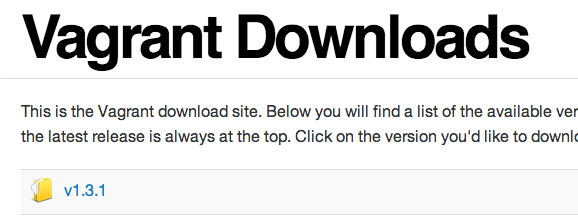
\includegraphics[width=\textwidth]{screenshots/Lesson1_2SS1.png}
\subsubsection*{3. Select the download/installer appropriate for your system. I chose dmg for my Mac OS X system.|}
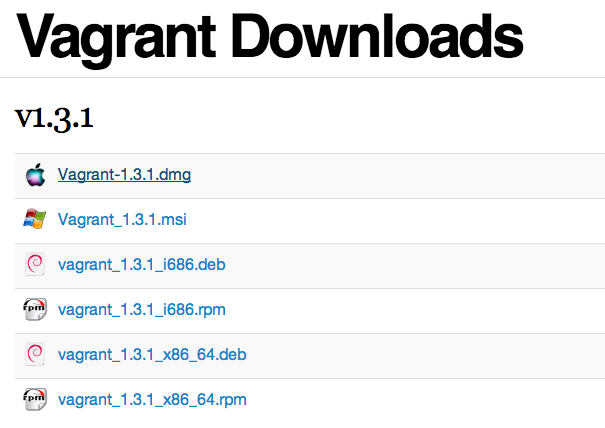
\includegraphics[width=\textwidth]{screenshots/Lesson1_2SS2.png}

\subsection{Setup the VM}
Now that Vagrant is installed we can install/setup our virtual machine with it.
\begin{enumerate}
  \item Execute the VirtualBox installer to install the software.
  \item Copy the \textbf{KFSDev.box} from the distributed USB drive to
    your hard disk.
  \item Execute from a shell 
    \begin{minted}{sh}
vagrant box add KFSDev https://dl.dropboxusercontent.com/u/883064/KFSDev.box
    \end{minted}
  \item Run init
    \begin{minted}{sh}
vagrant init KFSDev
    \end{minted}
  \item Import the Virtual Machine
    \begin{minted}{sh}
vagrant up
    \end{minted}
  \item Stop the Virtual Machine
    \begin{minted}{sh}
vagrant halt
    \end{minted}
  \item Start VirtualBox
\end{enumerate}

\subsection{Virtual Machine Manifest}
The VirtualBox appliance is an Ubuntu Linux distribution. Within it is
the software we will use for this class:
\begin{description}
  \item [Eclipse Indigo] the IDE used for class. Includes Subclipse,
    the m2eclipse plugin, and pre-installed projects with examples.
  \item [OpenJDK 1.7.0\_06 IcedTea] the JVM used for executing/testing
    examples.
  \item [Maven 3] used to build Rice applications, run tests, and
    start the Tomcat6 application
\end{description}

\subsubsection{Credentials}
\begin{description}
\item [User Account] is \textbf{kuali} with the password
  \textbf{kuali}. This is used to unlock the VM after it has suspended,
  gone to sleep, or locked. The password is also required for
  executing commands as \textbf{root} which may on occassion be
  required. The user account home directory is located at
  \textbf{/home/kuali} and will frequently be referred to during the training.
\item [Database Account] uses the jdbc connection string
  \textbf{jdbc:mysql://localhost:3306/kuldemo} and the
  username/password \textbf{kuldemo}/\textbf{kuldemo}. These are the
  default credentials and database connection information as defined
  in kul-cfg-dbs.
\end{description}

\subsubsection{Structure}
The Eclipse workspace is located at \textbf{/home/kuali/workspace}. 

\addcontentsline{toc}{section}{Setup Eclipse}
{\setlength{\baselineskip}%
  {0.0\baselineskip}
  \section*{\flushright Setup Eclipse}
  \hrulefill \par}

\subsection*{Setup Subclipse}
The Kuali Foundation currently standardizes on SVN as a version control system. Eclipse does not come with SVN support out-of-the box. We need to add it.
\subsubsection*{1. Go to the Eclipse Marketplace}
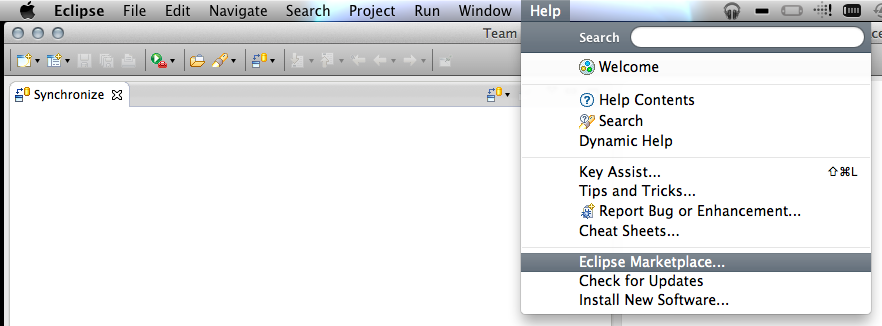
\includegraphics[width=\textwidth]{screenshots/Lesson1_2SS3.png}

\subsubsection*{2. Search for subclipse}
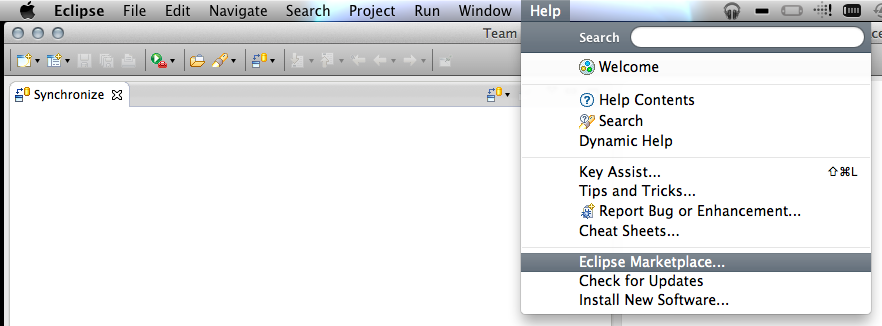
\includegraphics[width=\textwidth]{screenshots/Lesson1_2SS3.png}

\subsubsection*{3. Click the install button}
It's all downhill from here. 

\subsubsection*{4. Restart eclipse}

\subsection*{Add KFS Training Course SVN Repository}
We will be using this repository for course files as we progress.

\subsubsection*{1. Select 'Other' views}
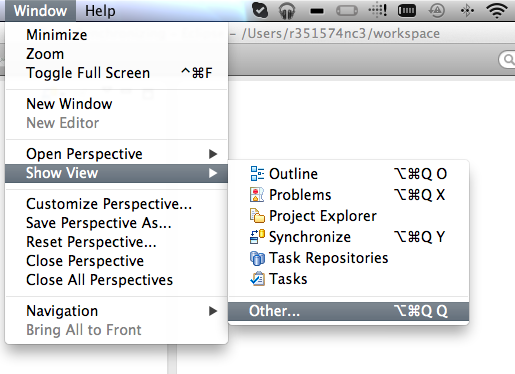
\includegraphics[width=\textwidth]{screenshots/Lesson1_2SS5.png}

\subsubsection*{2. Choose SVN Repositories}
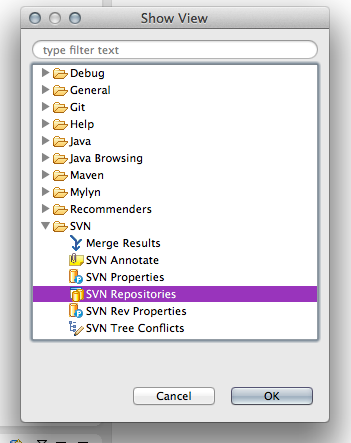
\includegraphics[width=\textwidth]{screenshots/Lesson1_2SS6.png}

\subsubsection*{3. Click the ``Add a SVN Repository'' Button}
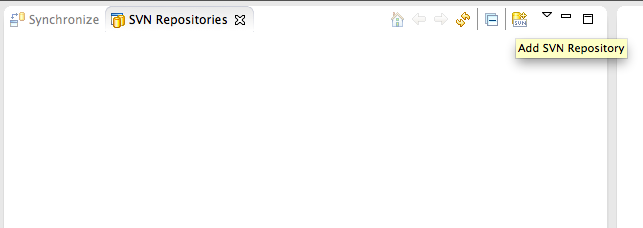
\includegraphics[width=\textwidth]{screenshots/Lesson1_2SS7.png}

\subsubsection*{4. Add the KFS Training SVN Repository URL}
Use \url{https://kfs-training.googlecode.com/svn/branches/4.1.1/}

\subsubsection*{5. Click the ``Finish'' Button}
That's it. There are no credentials here because we'll be using this
repository anonymously.

\addcontentsline{toc}{section}{Database Setup}
{\setlength{\baselineskip}%
  {0.0\baselineskip}
  \section*{\flushright Database Setup}
  \hrulefill \par}

\addcontentsline{toc}{subsection}{Instructions}
\subsection*{Instructions}
\subsubsection*{1 Update impex-build.properties}
Open \textbf{/home/kuali/workspace/impex-build.properties}. Locate the section of code that looks like
\begin{minted}{yaml}
import.torque.database = mysql
import.torque.database.driver = com.mysql.jdbc.Driver
import.torque.database.url = jdbc:mysql://localhost:3306/kuldemo
import.torque.database.user=kuldemo
import.torque.database.schema=KULDEMO
import.torque.database.password=kuldemo
\end{minted}

and change it to

\begin{minted}{yaml}
import.torque.database = mysql
import.torque.database.driver = com.mysql.jdbc.Driver
import.torque.database.url = jdbc:mysql://localhost:3306/kuldev
import.torque.database.user=kuldev
import.torque.database.schema=KULDEV
import.torque.database.password=kuldev
\end{minted}

\subsubsection{1 Update kfs-build.properties}
Open \textbf{/home/kuali/workspace/kfs-build.properties} Locate the section of code that looks like
\begin{minted}{yaml}
datasource.username=kuldemo
datasource.password=kuldemo
mysql.datasource.url=jdbc:mysql://localhost:3306/kuldemo
\end{minted}

and change it to

\begin{minted}{yaml}
datasource.username=kuldev
datasource.password=kuldev
mysql.datasource.url=jdbc:mysql://localhost:3306/KULDEV
\end{minted}

\subsubsection{2 Run Impex}
Using a terminal window do the following:
\begin{minted}{sh}
cd /home/kuali/workspace/kul-cfg-dbs/impex
ant -Dimpex.properties.file=$HOME/workspace/impex-build.properties \
    drop-schema create-schema import
\end{minted}

\end{document}